\documentclass[11pt,a4paper]{report}
\usepackage[textwidth=37em,vmargin=30mm]{geometry}
\usepackage{calc,xunicode,amsmath,amssymb,paralist,enumitem,tabu,booktabs,datetime2,xeCJK,xeCJKfntef,listings}
\usepackage{tocloft,fancyhdr,tcolorbox,xcolor,graphicx,eso-pic,xltxtra,xelatexemoji}

\newcommand{\envyear}[0]{2025}
\newcommand{\envdatestr}[0]{2025-03-28}
\newcommand{\envfinaldir}[0]{webdb/2025/20250328/final}

\usepackage[hidelinks]{hyperref}
\hypersetup{
    colorlinks=false,
    pdfpagemode=FullScreen,
    pdftitle={Web Digest - \envdatestr}
}

\setlength{\cftbeforechapskip}{10pt}
\renewcommand{\cftchapfont}{\rmfamily\bfseries\large\raggedright}
\setlength{\cftbeforesecskip}{2pt}
\renewcommand{\cftsecfont}{\sffamily\small\raggedright}

\setdefaultleftmargin{2em}{2em}{1em}{1em}{1em}{1em}

\usepackage{xeCJK,xeCJKfntef}
\xeCJKsetup{PunctStyle=plain,RubberPunctSkip=false,CJKglue=\strut\hskip 0pt plus 0.1em minus 0.05em,CJKecglue=\strut\hskip 0.22em plus 0.2em}
\XeTeXlinebreaklocale "zh"
\XeTeXlinebreakskip = 0pt


\setmainfont{Brygada 1918}
\setromanfont{Brygada 1918}
\setsansfont{IBM Plex Sans}
\setmonofont{JetBrains Mono NL}
\setCJKmainfont{Noto Serif CJK SC}
\setCJKromanfont{Noto Serif CJK SC}
\setCJKsansfont{Noto Sans CJK SC}
\setCJKmonofont{Noto Sans CJK SC}

\setlength{\parindent}{0pt}
\setlength{\parskip}{8pt}
\linespread{1.15}

\lstset{
	basicstyle=\ttfamily\footnotesize,
	numbersep=5pt,
	backgroundcolor=\color{black!5},
	showspaces=false,
	showstringspaces=false,
	showtabs=false,
	tabsize=2,
	captionpos=b,
	breaklines=true,
	breakatwhitespace=true,
	breakautoindent=true,
	linewidth=\textwidth
}






\newcommand{\coverpic}[2]{
    % argv: itemurl, authorname
    Cover photo by #2~~(\href{#1}{#1})
}
\newcommand{\makeheader}[0]{
    \begin{titlepage}
        % \newgeometry{hmargin=15mm,tmargin=21mm,bmargin=12mm}
        \begin{center}
            
            \rmfamily\scshape
            \fontspec{BaskervilleF}
            \fontspec{Old Standard}
            \fontsize{59pt}{70pt}\selectfont
            WEB\hfill DIGEST
            
            \vfill
            % \vskip 30pt
            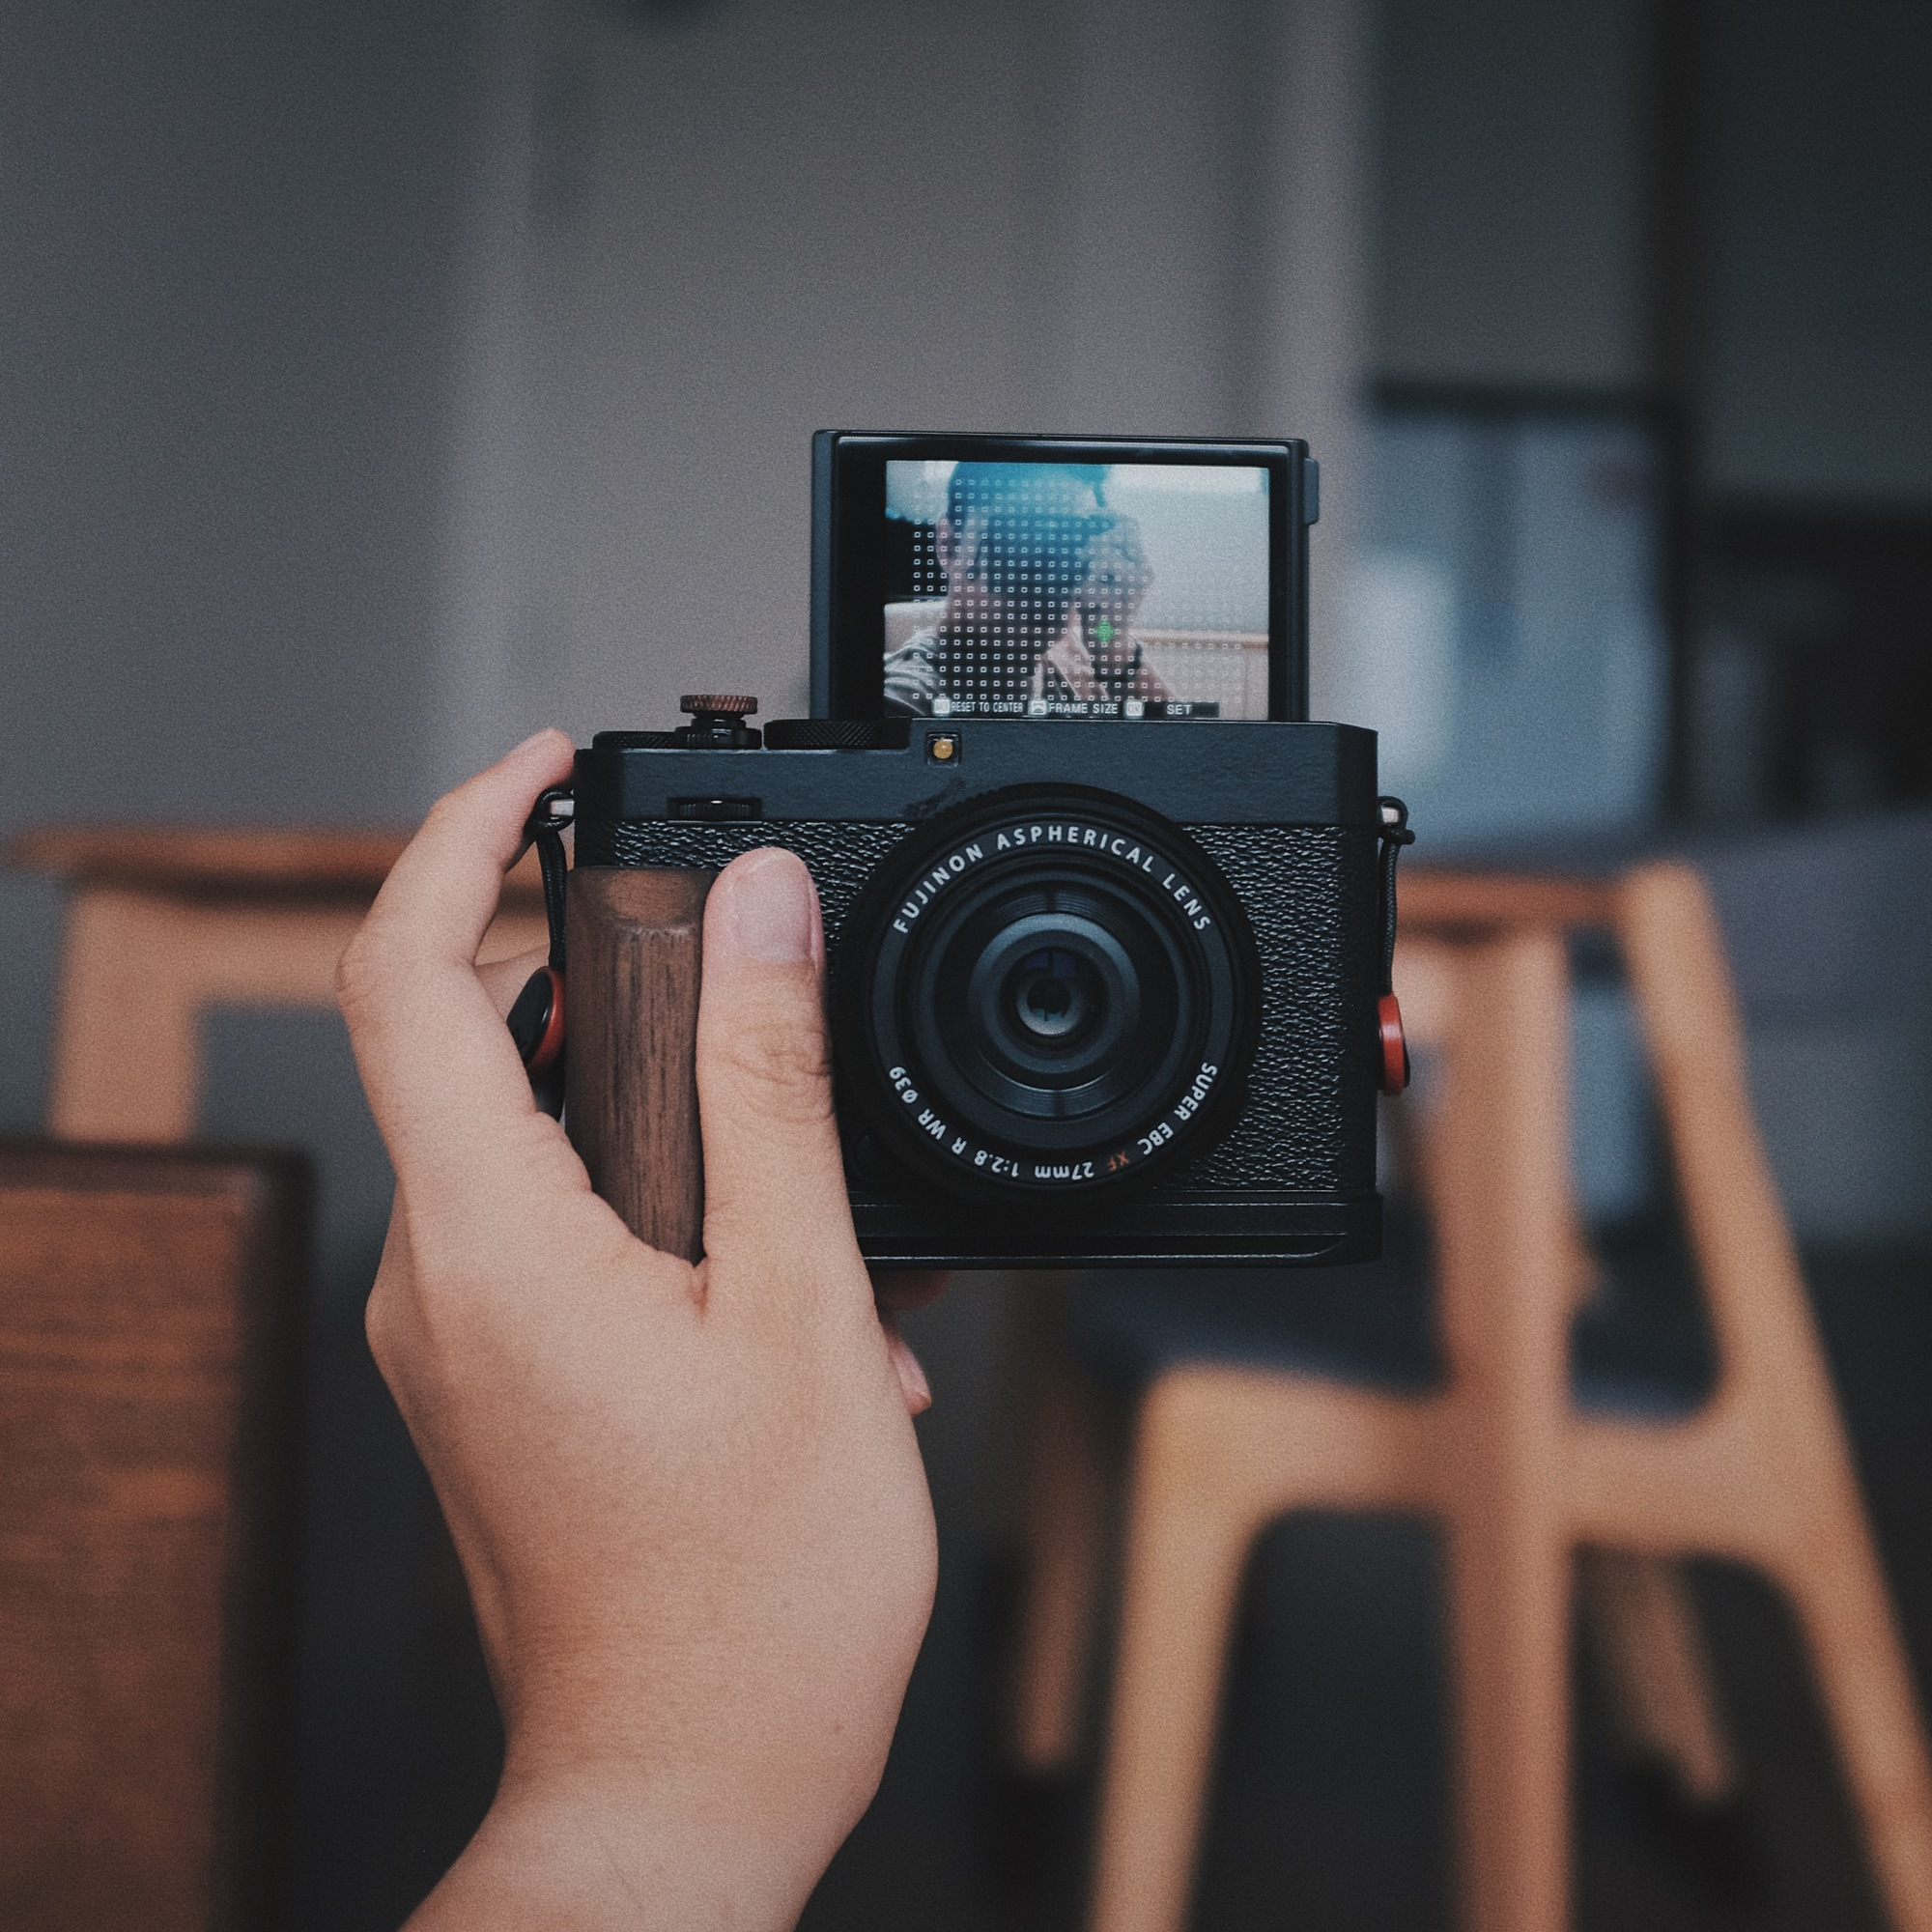
\includegraphics[width=\linewidth]{\envfinaldir/coverpic-prod.jpg}\par
            % \vskip 30pt
            \vfill

            \normalsize\rmfamily\scshape
            \copyright{} The Web Digest Project \hfill\large \envdatestr
        \end{center}
    \end{titlepage}
    % \restoregeometry
}
\newcommand{\simplehref}[1]{%
    \textcolor{blue!80!green}{\href{#1}{#1}}%
}
\renewcommand{\contentsname}{\center\Huge\sffamily\bfseries Contents\par\vskip 20pt}
\newcounter{ipartcounter}
\setcounter{ipartcounter}{0}
\newcommand{\ipart}[1]{
    % \vskip 20pt
    \clearpage
    \stepcounter{ipartcounter}
    \phantomsection
    \addcontentsline{toc}{chapter}{#1}
    % \begin{center}
    %     \Huge
    %     \sffamily\bfseries
    %     #1
    % \end{center}
    % \vskip 20pt plus 7pt
}
\newcounter{ichaptercounter}
\setcounter{ichaptercounter}{0}
\newcommand{\ichapter}[1]{
    % \vskip 20pt
    \clearpage
    \stepcounter{ichaptercounter}
    \phantomsection
    \addcontentsline{toc}{section}{\numberline{\arabic{ichaptercounter}}#1}
    \begin{center}
        \Huge
        \sffamily\bfseries
        #1
    \end{center}
    \vskip 20pt plus 7pt
}
\newcommand{\entrytitlefont}[1]{\subsection*{\raggedright\Large\sffamily\bfseries#1}}
\newcommand{\entryitemGeneric}[2]{
    % argv: title, url
    \parbox{\linewidth}{
        \entrytitlefont{#1}\par\vskip 5pt
        \footnotesize\ttfamily\mdseries
        \simplehref{#2}
    }\vskip 11pt plus 11pt minus 1pt
}
\newcommand{\entryitemGithub}[3]{
    % argv: title, url, desc
    \parbox{\linewidth}{
        \entrytitlefont{#1}\par\vskip 5pt
        \footnotesize\ttfamily\mdseries
        \simplehref{#2}\par\vskip 5pt
        \small\rmfamily\mdseries#3
    }\vskip 11pt plus 11pt minus 1pt
}
\newcommand{\entryitemAp}[3]{
    % argv: title, url, desc
    \parbox{\linewidth}{
        \entrytitlefont{#1}\par\vskip 5pt
        \footnotesize\ttfamily\mdseries
        \simplehref{#2}\par\vskip 5pt
        \small\rmfamily\mdseries#3
    }\vskip 11pt plus 11pt minus 1pt
}
\newcommand{\entryitemHackernews}[3]{
    % argv: title, hnurl, rawurl
    % \parbox{\linewidth}{
    %     \entrytitlefont{#1}\par\vskip 5pt
    %     \footnotesize\ttfamily\mdseries
    %     \simplehref{#3}\par
    %     \textcolor{black!50}{\href{#2}{#2}}
    % }\vskip 11pt plus 11pt minus 1pt
    \begin{minipage}{\linewidth}
            \entrytitlefont{#1}\par\vskip 5pt
            \footnotesize\ttfamily\mdseries
            \simplehref{#3}\par
            \textcolor{black!50}{\href{#2}{#2}}
    \end{minipage}\par\vskip 11pt plus 11pt minus 1pt
}







\begin{document}

\makeheader

\tableofcontents\clearpage




\ipart{Developers}
\ichapter{Hacker News}
\entryitemTwoLinks{Apple needs a Snow Sequoia}{https://news.ycombinator.com/item?id=43498984}{https://reviews.ofb.biz/safari/article/1300.html}

\entryitemTwoLinks{How to Use Em Dashes (–), En Dashes (–), and Hyphens (-)}{https://news.ycombinator.com/item?id=43497719}{https://www.merriam-webster.com/grammar/em-dash-en-dash-how-to-use}

\entryitemTwoLinks{I tried making artificial sunlight at home}{https://news.ycombinator.com/item?id=43497394}{https://victorpoughon.fr/i-tried-making-artificial-sunlight-at-home/}

\entryitemTwoLinks{SignalGate Is Driving the Most US Downloads of Signal Ever}{https://news.ycombinator.com/item?id=43497150}{https://www.wired.com/story/signalgate-is-driving-the-most-us-downloads-of-signal-ever/}

\entryitemTwoLinks{AI models miss disease in Black and female patients}{https://news.ycombinator.com/item?id=43496644}{https://www.science.org/content/article/ai-models-miss-disease-black-female-patients}

\entryitemTwoLinks{California bill aims to phase out harmful ultra-processed foods in schools}{https://news.ycombinator.com/item?id=43495997}{https://www.thenewlede.org/2025/03/california-bill-aims-to-phase-out-harmful-ultra-processed-foods-in-schools/}

\entryitemTwoLinks{Abundance Isn't Going to Happen Unless Politicians Are Scared of the Status Quo}{https://news.ycombinator.com/item?id=43495644}{https://inpractice.yimbyaction.org/p/abundance-isnt-going-to-happen-unless}

\entryitemTwoLinks{Tracing the thoughts of a large language model}{https://news.ycombinator.com/item?id=43495617}{https://www.anthropic.com/research/tracing-thoughts-language-model}

\entryitemTwoLinks{Zoom bias: The social costs of having a 'tinny' sound during video conferences}{https://news.ycombinator.com/item?id=43495465}{https://phys.org/news/2025-03-bias-social-tinny-video-conferences.html}

\entryitemTwoLinks{Launch HN: Continue (YC S23) – Create custom AI code assistants}{https://news.ycombinator.com/item?id=43494427}{https://hub.continue.dev/explore/assistants}

\entryitemTwoLinks{A filmmaker and a crooked lawyer shattered Denmark's self-image}{https://news.ycombinator.com/item?id=43493159}{https://www.theguardian.com/world/2025/mar/27/black-swan-denmark-documentary-mads-brugger-amira-smajic}

\entryitemTwoLinks{Blasting Past WebP - An analysis of the NSO BLASTPASS iMessage exploit}{https://news.ycombinator.com/item?id=43493056}{https://googleprojectzero.blogspot.com/2025/03/blasting-past-webp.html}

\entryitemTwoLinks{Source code art in the Rivulet language}{https://news.ycombinator.com/item?id=43492652}{https://github.com/rottytooth/Rivulet}

\entryitemTwoLinks{Piranesi's Perspective Trick (2019)}{https://news.ycombinator.com/item?id=43492562}{https://medium.com/@brunopostle/piranesis-perspective-trick-6bcd7a754da9}

\entryitemTwoLinks{Modern C}{https://news.ycombinator.com/item?id=43492211}{https://gustedt.gitlabpages.inria.fr/modern-c/}

\entryitemTwoLinks{Glider for Apple II}{https://news.ycombinator.com/item?id=43491977}{https://www.colino.net/wordpress/en/glider-for-apple-ii/}

\entryitemTwoLinks{They Might Be Giants Flood EPK Promo (1990) [video]}{https://news.ycombinator.com/item?id=43490173}{https://www.youtube.com/watch?v=C-tQSFQ-ESY}

\entryitemTwoLinks{DeepSeek-V3 Technical Report}{https://news.ycombinator.com/item?id=43490167}{https://arxiv.org/abs/2412.19437}

\entryitemTwoLinks{DJ With Apple Music launches to enable subscribers to mix their own sets}{https://news.ycombinator.com/item?id=43489271}{https://www.musicweek.com/digital/read/dj-with-apple-music-launches-to-enable-subscribers-to-mix-their-own-sets/091655}

\entryitemTwoLinks{The mysterious flow of fluid in the brain}{https://news.ycombinator.com/item?id=43489136}{https://www.quantamagazine.org/the-mysterious-flow-of-fluid-in-the-brain-20250326/}\ichapter{Phoronix}
\entryitemGeneric{\hskip 0pt{}Linux 6.15 SoC/DT Additions: Arm Morello, Versal NET, Apple T2, MNT Reform 2 \& More}{https://www.phoronix.com/news/Linux-6.15-SoC-DT-Updates}

\entryitemGeneric{\hskip 0pt{}Ubuntu 25.04 Beta Officially Released}{https://www.phoronix.com/news/Ubuntu-25.04-Beta}

\entryitemGeneric{\hskip 0pt{}EXT4 Better Hardened Against Maliciously-Fuzzed File-Systems}{https://www.phoronix.com/news/Linux-6.15-EXT4}

\entryitemGeneric{\hskip 0pt{}Ubuntu 25.04 Beta Delivering Some Nice Performance Improvements Over Ubuntu 24.10}{https://www.phoronix.com/review/ubuntu-2504-beta-benchmarks}

\entryitemGeneric{\hskip 0pt{}Akamai Now Providing The Hosting Infrastructure For Kernel.org}{https://www.phoronix.com/news/Akamai-Hosting-Kernel.org}

\entryitemGeneric{\hskip 0pt{}Zstd 1.5.7 Lands In Linux 6.15 For Better Performance \& APIs For Intel QAT Acceleration}{https://www.phoronix.com/news/Zstd-1.5.7-In-Linux-6.15}

\entryitemGeneric{\hskip 0pt{}Linux 6.15 To Gain New Option For Those Building The Kernel Without Virtual Terminal}{https://www.phoronix.com/news/Linux-6.15-Null-TTY-Default}

\entryitemGeneric{\hskip 0pt{}PostgreSQL Database Lands Initial Support For IO\_uring: "Can Be Considerably Faster"}{https://www.phoronix.com/news/PostgreSQL-Lands-IO\_uring}

\entryitemGeneric{\hskip 0pt{}Linux 6.15 Brings Support For New Sound Hardware, Continued SoundWire Improvements}{https://www.phoronix.com/news/Linux-6.15-Sound}\ichapter{Dribbble}
\entryitemGeneric{\hskip 0pt{}Proven UI/UX design, User Interface experience}{https://dribbble.com/shots/25819444-Proven-UI-UX-design-User-Interface-experience}

\entryitemGeneric{\hskip 0pt{}Big gestures}{https://dribbble.com/shots/25826632-Big-gestures}

\entryitemGeneric{\hskip 0pt{}Dog + Play Button}{https://dribbble.com/shots/25809362-Dog-Play-Button}

\entryitemGeneric{\hskip 0pt{}Pricefy Logo Design - Mountains, Chart, Graph, Sun}{https://dribbble.com/shots/25824720-Pricefy-Logo-Design-Mountains-Chart-Graph-Sun}

\entryitemGeneric{\hskip 0pt{}Illustration}{https://dribbble.com/shots/25822720-Illustration}

\entryitemGeneric{\hskip 0pt{}Crypto Portfolio Tracker App}{https://dribbble.com/shots/25820014-Crypto-Portfolio-Tracker-App}

\entryitemGeneric{\hskip 0pt{}Gemini Rebrand}{https://dribbble.com/shots/25821410-Gemini-Rebrand}

\entryitemGeneric{\hskip 0pt{}Cyber Extrusion (Merch/Custom T-shirt)}{https://dribbble.com/shots/25821987-Cyber-Extrusion-Merch-Custom-T-shirt}

\entryitemGeneric{\hskip 0pt{}FCKD - Part 2}{https://dribbble.com/shots/25817864-FCKD-Part-2}

\entryitemGeneric{\hskip 0pt{}ROOT BEER}{https://dribbble.com/shots/25815759-ROOT-BEER}

\entryitemGeneric{\hskip 0pt{}Aura - Logo Design}{https://dribbble.com/shots/25815819-Aura-Logo-Design}

\entryitemGeneric{\hskip 0pt{}Complexure}{https://dribbble.com/shots/25815646-Complexure}

\entryitemGeneric{\hskip 0pt{}Snitcher - New Branding}{https://dribbble.com/shots/25816140-Snitcher-New-Branding}

\entryitemGeneric{\hskip 0pt{}Lepisov Branding Logo Reveal Animation}{https://dribbble.com/shots/25814536-Lepisov-Branding-Logo-Reveal-Animation}

\entryitemGeneric{\hskip 0pt{}Spark illustrations}{https://dribbble.com/shots/25815705-Spark-illustrations}

\entryitemGeneric{\hskip 0pt{}FCKD}{https://dribbble.com/shots/25812257-FCKD}

\entryitemGeneric{\hskip 0pt{}Spark}{https://dribbble.com/shots/25815686-Spark}

\entryitemGeneric{\hskip 0pt{}Spark illustrations}{https://dribbble.com/shots/25815717-Spark-illustrations}

\entryitemGeneric{\hskip 0pt{}Cimet Merch Car Wrapp}{https://dribbble.com/shots/25710572-Cimet-Merch-Car-Wrapp}

\entryitemGeneric{\hskip 0pt{}Revobyte Logo Design - R Letter / Monogram / Blockchain}{https://dribbble.com/shots/25811483-Revobyte-Logo-Design-R-Letter-Monogram-Blockchain}

\entryitemGeneric{\hskip 0pt{}S}{https://dribbble.com/shots/25814436-S}

\entryitemGeneric{\hskip 0pt{}Task completion micro interaction}{https://dribbble.com/shots/25797132-Task-completion-micro-interaction}

\entryitemGeneric{\hskip 0pt{}Phantom auto buy/sell concept}{https://dribbble.com/shots/25799751-Phantom-auto-buy-sell-concept}

\entryitemGeneric{\hskip 0pt{}Lumee Logo Design - iGaming / Gambling / Casino}{https://dribbble.com/shots/25801924-Lumee-Logo-Design-iGaming-Gambling-Casino}


\ipart{Developers~~~~(zh-Hans)}
\ichapter{Solidot}
\entryitemGeneric{\hskip 0pt{}Meta 考虑在英国推出无广告的付费订阅}{https://www.solidot.org/story?sid=80900}

\entryitemGeneric{\hskip 0pt{}Vivaldi 内置 Proton VPN }{https://www.solidot.org/story?sid=80899}

\entryitemGeneric{\hskip 0pt{}VMware 指控西门子盗版了它的软件}{https://www.solidot.org/story?sid=80898}

\entryitemGeneric{\hskip 0pt{}日本数学家首次赢得阿贝尔奖}{https://www.solidot.org/story?sid=80897}

\entryitemGeneric{\hskip 0pt{}高盐饮食在小鼠诱发类抑郁症状}{https://www.solidot.org/story?sid=80895}

\entryitemGeneric{\hskip 0pt{}日本公司推出太空葬服务}{https://www.solidot.org/story?sid=80894}

\entryitemGeneric{\hskip 0pt{}Android 最早从下周起进入封闭式开发,仍然会开源}{https://www.solidot.org/story?sid=80893}

\entryitemGeneric{\hskip 0pt{}比亚迪 2024 年销售收入超过特斯拉}{https://www.solidot.org/story?sid=80892}

\entryitemGeneric{\hskip 0pt{}火星发现长链有机分子}{https://www.solidot.org/story?sid=80891}

\entryitemGeneric{\hskip 0pt{}年轻一代的消费者更爱内容创作者而非传统电视电影}{https://www.solidot.org/story?sid=80889}

\entryitemGeneric{\hskip 0pt{}近半加拿大家庭完全停止消费有线电视}{https://www.solidot.org/story?sid=80888}

\entryitemGeneric{\hskip 0pt{} Infinite Reality 以 2.07 亿美元收购 Napster}{https://www.solidot.org/story?sid=80887}

\entryitemGeneric{\hskip 0pt{}H5N1 禽流感在英国传播到绵羊}{https://www.solidot.org/story?sid=80886}

\entryitemGeneric{\hskip 0pt{}火星东半球被认为蕴含丰富的冰}{https://www.solidot.org/story?sid=80885}

\entryitemGeneric{\hskip 0pt{}交通噪音会触发鸟类的路怒症}{https://www.solidot.org/story?sid=80884}

\entryitemGeneric{\hskip 0pt{}东京法庭下令解散统一教会}{https://www.solidot.org/story?sid=80883}

\entryitemGeneric{\hskip 0pt{}Game Informer 杂志复活}{https://www.solidot.org/story?sid=80882}

\entryitemGeneric{\hskip 0pt{}李开复称中美 AI 差距仅为三个月}{https://www.solidot.org/story?sid=80881}

\entryitemGeneric{\hskip 0pt{}科学家寻求更精确的测量疼痛}{https://www.solidot.org/story?sid=80880}

\entryitemGeneric{\hskip 0pt{}银河系中心的龙卷风}{https://www.solidot.org/story?sid=80879}\ichapter{V2EX}
\entryitemGeneric{\hskip 0pt{}[Android] 安卓平台目前有没有支持创建自定义规则的代理应用?}{https://www.v2ex.com/t/1121648}

\entryitemGeneric{\hskip 0pt{}[智能家电] 25 年 4 月,求推荐 85 寸电视,价格 1.2w 左右}{https://www.v2ex.com/t/1121647}

\entryitemGeneric{\hskip 0pt{}[程序员] (帖子有点长)有这样的面试官得物凭什么做第一技术梯队的梦? 关于我在得物中间件组的一次糟糕面试经历.}{https://www.v2ex.com/t/1121646}

\entryitemGeneric{\hskip 0pt{}[全球工单系统] 谨慎升级微信 Mac 版 4.0.3 Beta,会丢失许多聊天记录}{https://www.v2ex.com/t/1121645}

\entryitemGeneric{\hskip 0pt{}[宽带症候群] 请教大佬们:网络工程师入门,公司 \& 职位怎么选?}{https://www.v2ex.com/t/1121644}

\entryitemGeneric{\hskip 0pt{}[macOS] dock 栏两个应用图标之间有个白点}{https://www.v2ex.com/t/1121643}

\entryitemGeneric{\hskip 0pt{}[NAS] n150 的性能是物理飞牛还是虚拟飞牛?}{https://www.v2ex.com/t/1121642}

\entryitemGeneric{\hskip 0pt{}[生活] 有了小孩之后,人会变得更加怕死吗?}{https://www.v2ex.com/t/1121640}

\entryitemGeneric{\hskip 0pt{}[问与答] 一直正常使用的梯子突然发现 Google Play 商店下载 App 速度非常慢该怎么解决}{https://www.v2ex.com/t/1121639}

\entryitemGeneric{\hskip 0pt{}[Apple] iCloud 如何选择部分相集自动同步}{https://www.v2ex.com/t/1121638}

\entryitemGeneric{\hskip 0pt{}[iOS] App Store,下架国区的 App,有更新提示,但是无法更新}{https://www.v2ex.com/t/1121637}

\entryitemGeneric{\hskip 0pt{}[分享创造] 重复造轮子之写了一个基于 ai 生成 git 提交信息的命令行工具}{https://www.v2ex.com/t/1121636}

\entryitemGeneric{\hskip 0pt{}[Android] 求一个将手机设定为网关的方法}{https://www.v2ex.com/t/1121635}

\entryitemGeneric{\hskip 0pt{}[宽带症候群] 上行带宽这么小是阴谋吗?}{https://www.v2ex.com/t/1121632}

\entryitemGeneric{\hskip 0pt{}[问与答] 有什么办法解决应用上架所需的``特殊资质''限制?}{https://www.v2ex.com/t/1121629}

\entryitemGeneric{\hskip 0pt{}[深圳] 上班在深圳前海湾, 附近有一室一厅的房子推荐吗}{https://www.v2ex.com/t/1121628}

\entryitemGeneric{\hskip 0pt{}[推广] [开奖结果] 恭喜 15 位幸运儿,你们中奖啦!快来领奖!}{https://www.v2ex.com/t/1121627}

\entryitemGeneric{\hskip 0pt{}[投资] 有一起交流学习量化的兄弟吗?}{https://www.v2ex.com/t/1121626}

\entryitemGeneric{\hskip 0pt{}[云计算] OSS 签名绕过上传任意文件到别人的网站}{https://www.v2ex.com/t/1121625}

\entryitemGeneric{\hskip 0pt{}[推广] gpt-4o-all 支持 openai 最新的画图和编辑图片功能}{https://www.v2ex.com/t/1121621}

\entryitemGeneric{\hskip 0pt{}[全球工单系统] 一个关于微信的神奇 BUG}{https://www.v2ex.com/t/1121620}

\entryitemGeneric{\hskip 0pt{}[海外留学] 忙活了这么长时间终于有个结果,悄悄发在这里}{https://www.v2ex.com/t/1121618}

\entryitemGeneric{\hskip 0pt{}[酷工作] [杭州] 支付宝招前端!急急急}{https://www.v2ex.com/t/1121617}

\entryitemGeneric{\hskip 0pt{}[新手求助] v2ex 编辑帖子好贵啊!}{https://www.v2ex.com/t/1121614}

\entryitemGeneric{\hskip 0pt{}[Apple] 苹果的 Passwords 如何只存 2FA?}{https://www.v2ex.com/t/1121613}

\entryitemGeneric{\hskip 0pt{}[Android] Tips: 给不支持语言偏好列表的国产安卓(如 MIUI)设置语言偏好(需 ROOT)}{https://www.v2ex.com/t/1121612}

\entryitemGeneric{\hskip 0pt{}[分享发现] 现在做付费应用,都不一定要接入支付系统了。}{https://www.v2ex.com/t/1121611}

\entryitemGeneric{\hskip 0pt{}[宽带症候群] 三大运营商互访,夜间爆炸厉害,难道要靠日本服务器/阿里云 200M 来拯救了吗?}{https://www.v2ex.com/t/1121610}

\entryitemGeneric{\hskip 0pt{}[程序员] 技术栈选择: Java 还是 Python}{https://www.v2ex.com/t/1121609}

\entryitemGeneric{\hskip 0pt{}[随想] 最近在杞人忧天的考虑一个问题}{https://www.v2ex.com/t/1121608}

\entryitemGeneric{\hskip 0pt{}[Docker] 小白请教 docker 安装后出现的问题}{https://www.v2ex.com/t/1121607}

\entryitemGeneric{\hskip 0pt{}[问与答] QQ 截图颜色差异问题}{https://www.v2ex.com/t/1121606}

\entryitemGeneric{\hskip 0pt{}[问与答] 你们看完一篇文章能把握住内容细节吗?}{https://www.v2ex.com/t/1121605}

\entryitemGeneric{\hskip 0pt{}[macOS] 原来在开发者将 iPadOS 的 App 从 Mac App Store 下架后,已经在 Mac 安装的 App 也无法运行了}{https://www.v2ex.com/t/1121602}

\entryitemGeneric{\hskip 0pt{}[问与答] 个人怎么申请 shopee 的开放平台账号?}{https://www.v2ex.com/t/1121601}

\entryitemGeneric{\hskip 0pt{}[Android] 小米 HyperOS 使用 Bitwarden 管理 passkey}{https://www.v2ex.com/t/1121600}

\entryitemGeneric{\hskip 0pt{}[分享创造] 用 PyQt 搞了个日历笔记本}{https://www.v2ex.com/t/1121599}

\entryitemGeneric{\hskip 0pt{}[Apple] Videoer - 视频格式转换工具,支持 MP4、MKV、MOV、AVI、GIF 等格式互转,轻松处理批量文件!还支持音频提取、字幕添加}{https://www.v2ex.com/t/1121598}

\entryitemGeneric{\hskip 0pt{}[问与答] 喜欢酒桶形机械表,求推荐牌子, 2000 以内}{https://www.v2ex.com/t/1121597}

\entryitemGeneric{\hskip 0pt{}[投资] 离开 A 股 10 天回来,一切都不一样,离开 10 年回来,一切都一样}{https://www.v2ex.com/t/1121596}

\entryitemGeneric{\hskip 0pt{}[PayPal] 请问 paypal 提现到香港中国银行要如何填写}{https://www.v2ex.com/t/1121595}

\entryitemGeneric{\hskip 0pt{}[分享发现] [注册即送 1GB] 海外代理池 + 爬虫采集 API}{https://www.v2ex.com/t/1121594}

\entryitemGeneric{\hskip 0pt{}[Apple TV] 为什么 apple tv + 只有电视端需要走代理?}{https://www.v2ex.com/t/1121593}

\entryitemGeneric{\hskip 0pt{}[问与答] 笔记本选购求推荐}{https://www.v2ex.com/t/1121592}

\entryitemGeneric{\hskip 0pt{}[问与答] 如何制作自己的电子书,并打印成 A6 的本子(求当前最佳实践方案}{https://www.v2ex.com/t/1121591}

\entryitemGeneric{\hskip 0pt{}[问与答] 以前视频网站都流行的关灯效果,近些年怎么看不到了?}{https://www.v2ex.com/t/1121590}

\entryitemGeneric{\hskip 0pt{}[macOS] 15 年的 mba,挂海鲜市场卖了 500,如果不卖,还有啥用途?换个电池搭配显示器家用,可行吗?}{https://www.v2ex.com/t/1121589}

\entryitemGeneric{\hskip 0pt{}[问与答] 有没有好用的工具,能把视频中的语音全部转成文字?}{https://www.v2ex.com/t/1121588}

\entryitemGeneric{\hskip 0pt{}[生活] 不吐不快: 当今环境下普通人出售自有房或车就是一种修行}{https://www.v2ex.com/t/1121587}

\entryitemGeneric{\hskip 0pt{}[git] 请教各位关于 Git 合并的问题}{https://www.v2ex.com/t/1121586}


\ipart{Generic News}
\ichapter{AP News}
\entryitemWithDescription{\hskip 0pt{}Ella Langley leads 2025 ACM Awards nominations. Beyoncé and Miranda Lambert are shut out}{https://apnews.com/article/627254ce15387577638370bb61a15ae5}{}

\entryitemWithDescription{\hskip 0pt{}Maine school officials won't comply with Trump administration agreement to bar transgender athletes}{https://apnews.com/article/e1f7232307fa400ac58d3471cd86b133}{}

\entryitemWithDescription{\hskip 0pt{}What to know after Prince Harry resigned from his African charity}{https://apnews.com/article/ca9a9b84e64ce07df4e1b0ad81665ee3}{}

\entryitemWithDescription{\hskip 0pt{}One Tech Tip: Don't give your email to strangers, use a decoy address instead}{https://apnews.com/article/5305c01c66b7ff67c2464d83fcf2a9d8}{}

\entryitemWithDescription{\hskip 0pt{}Will Smith gets street named in Philadelphia neighborhood where he was born and raised}{https://apnews.com/article/b84d2f19e88b9015c801d5ad59f2c673}{}

\entryitemWithDescription{\hskip 0pt{}30 years after music icon Selena's murder, Yolanda Saldívar is up for parole. Here's what to know}{https://apnews.com/article/c68df5e4f1e6398a54587044f35e652e}{}

\entryitemWithDescription{\hskip 0pt{}World Series champion LA Dodgers say they'll visit Trump at the White House on April 7}{https://apnews.com/article/fcf01550c4aee53039aa82fc88a7fe31}{}

\entryitemWithDescription{\hskip 0pt{}A new Chili's near Scranton will be a throwback to `The Office,' `awesome blossom' and all}{https://apnews.com/article/2faea0e7841dcd6903a798064fd17508}{}

\entryitemWithDescription{\hskip 0pt{}It was bacteria — not a miracle — on a Communion wafer in Indiana church}{https://apnews.com/article/fb90923979d6048dfacbacb65f11783f}{}

\entryitemWithDescription{\hskip 0pt{}Pilot and 2 young daughters survive the night on airplane wing after crashing into icy Alaska lake}{https://apnews.com/article/f385057ebd03c32cd6d766d2c521e856}{}

\entryitemWithDescription{\hskip 0pt{}Escaped otters cavort in the snow as the zoo's search continues}{https://apnews.com/article/937ee002eeced882e96b93ba36f16874}{}

\entryitemWithDescription{\hskip 0pt{}Texas Rep. Jasmine Crockett mocks Greg Abbott, who uses a wheelchair, as `Gov. Hot Wheels'}{https://apnews.com/article/a38d50b41e35cc6e05f5d72ad74ff54f}{}

\entryitemWithDescription{\hskip 0pt{}Kroger blames Albertsons for merger's demise in new court filings}{https://apnews.com/article/a93ae5b43e705c5350695c071a06331f}{}






\clearpage
\leavevmode\vfill
\footnotesize

Copyright \copyright{} 2023-2025 Neruthes and other contributors.

This document is published with CC BY-NC-ND 4.0 license.

The entries listed in this newsletter may be copyrighted by their respective creators.

This newsletter is generated by the Web Digest project.

The newsletters are also delivered via Telegram channel \CJKunderline{\href{https://t.me/webdigestchannel}{https://t.me/webdigestchannel}}.\\
RSS feed is available at \CJKunderline{\href{https://webdigest.pages.dev/rss.xml}{https://webdigest.pages.dev/rss.xml}}.

This newsletter is available in PDF at
\CJKunderline{\href{https://webdigest.pages.dev/}{https://webdigest.pages.dev/}}.

The source code being used to generate this newsletter is available at\\
\CJKunderline{\href{https://github.com/neruthes/webdigest}{https://github.com/neruthes/webdigest}}.

This newsletter is also available in
\CJKunderline{\href{http://webdigest.pages.dev/readhtml/\envyear/WebDigest-20250328.html}{HTML}} and
\CJKunderline{\href{https://github.com/neruthes/webdigest/blob/master/markdown/\envyear/WebDigest-20250328.md}{Markdown}}.


\coverpic{https://unsplash.com/photos/a-group-of-boats-sitting-on-top-of-a-beach-0B99fhgAuKA}{Cat Guffin}


\end{document}
